%# -*- coding: utf-8-unix -*-
%%==================================================
%% thesis.tex
%%==================================================

% 双面打印
%\documentclass[doctor, fontset=adobe, openright, twoside, zihao=-4]{sjtuthesis}
 \documentclass[bachelor, fontset=adobe, openany, oneside, zihao=-4, submit]{sjtuthesis} 
% \documentclass[master, adobefonts, review]{sjtuthesis} 
% \documentclass[%
%   bachelor|master|doctor,	% 必选项
%   fontset=adobe|windows,  	% 只测试了adobe
%   oneside|twoside,		% 单面打印,双面打印(奇偶页交换页边距,默认)
%   openany|openright, 		% 可以在奇数或者偶数页开新章|只在奇数页开新章(默认)
%   zihao=-4|5,, 		% 正文字号:小四、五号(默认)
%   review,	 		% 盲审论文,隐去作者姓名、学号、导师姓名、致谢、发表论文和参与的项目
%   submit			% 定稿提交的论文,插入签名扫描版的原创性声明、授权声明 
% ]

% 逐个导入参考文献数据库
\addbibresource{bib/thesis.bib}
% \addbibresource{bib/chap2.bib}

\begin{document}

%% 无编号内容:中英文论文封面、授权页
%# -*- coding: utf-8-unix -*-
\title{中国未来正负电子对撞机上希格斯相关物理的预研}
\author{张宇雷}
\advisor{李亮教授}
% \coadvisor{某某教授}
\defenddate{2016年06月01日}
\school{上海交通大学}
\institute{物理与天文系}
\studentnumber{5120729057}
\major{物理学(国际班)}

\englishtitle{Higgs Production Study at $\nu{\nu}H$ Channel with the future CEPC detector}
\englishauthor{\textsc{Yulei Zhang}}
\englishadvisor{Prof. \textsc{Liang Li}}
% \englishcoadvisor{Prof. \textsc{Uom Uom}}
\englishschool{Shanghai Jiao Tong University}
\englishinstitute{\textsc{Depart of Physics and Astronomy} \\
  \textsc{Shanghai Jiao Tong University} \\
  \textsc{Shanghai, P.R.China}}
\englishmajor{Physics(Internetional Class)}
\englishdate{Jun. 1st, 2016}


\maketitle

\makeenglishtitle

\makeatletter
\ifsjtu@submit\relax
	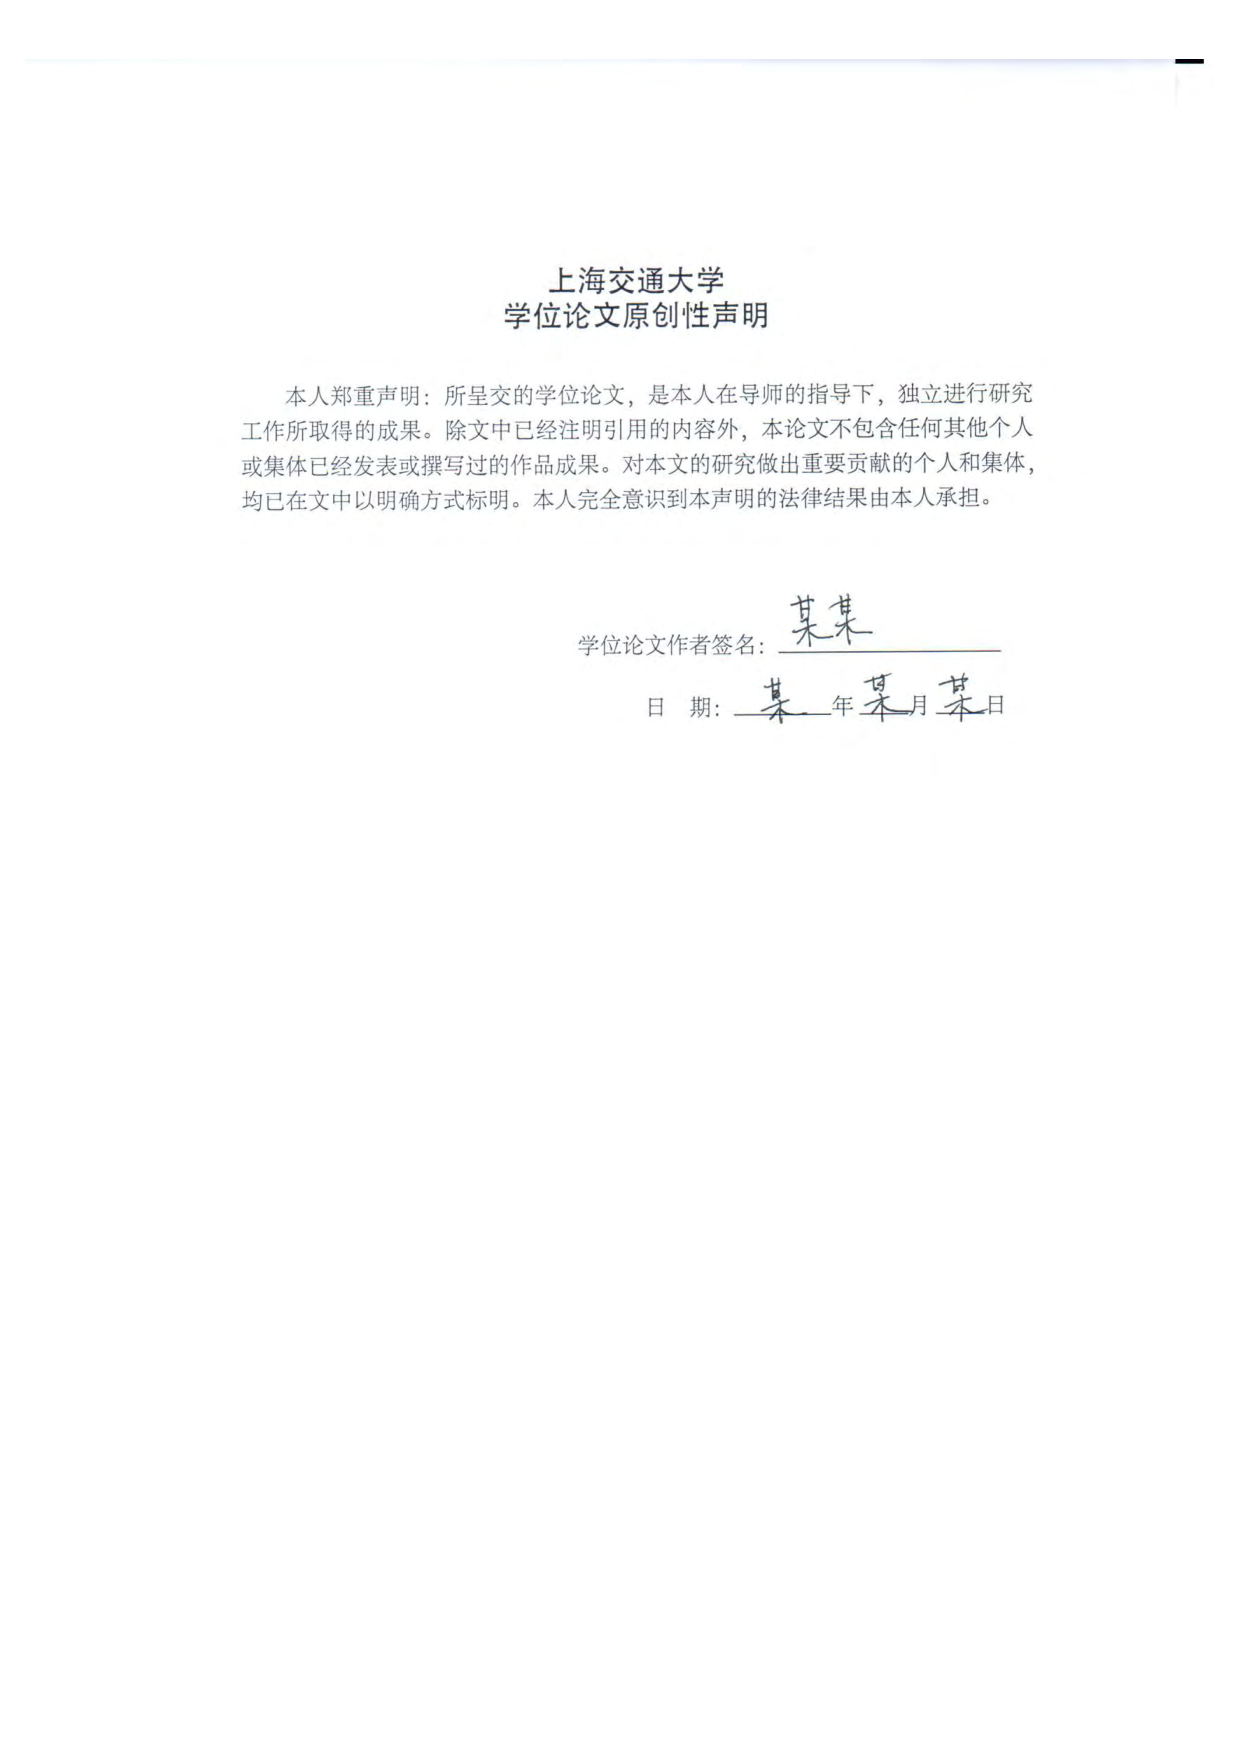
\includepdf{pdf/original.pdf}
	\cleardoublepage
	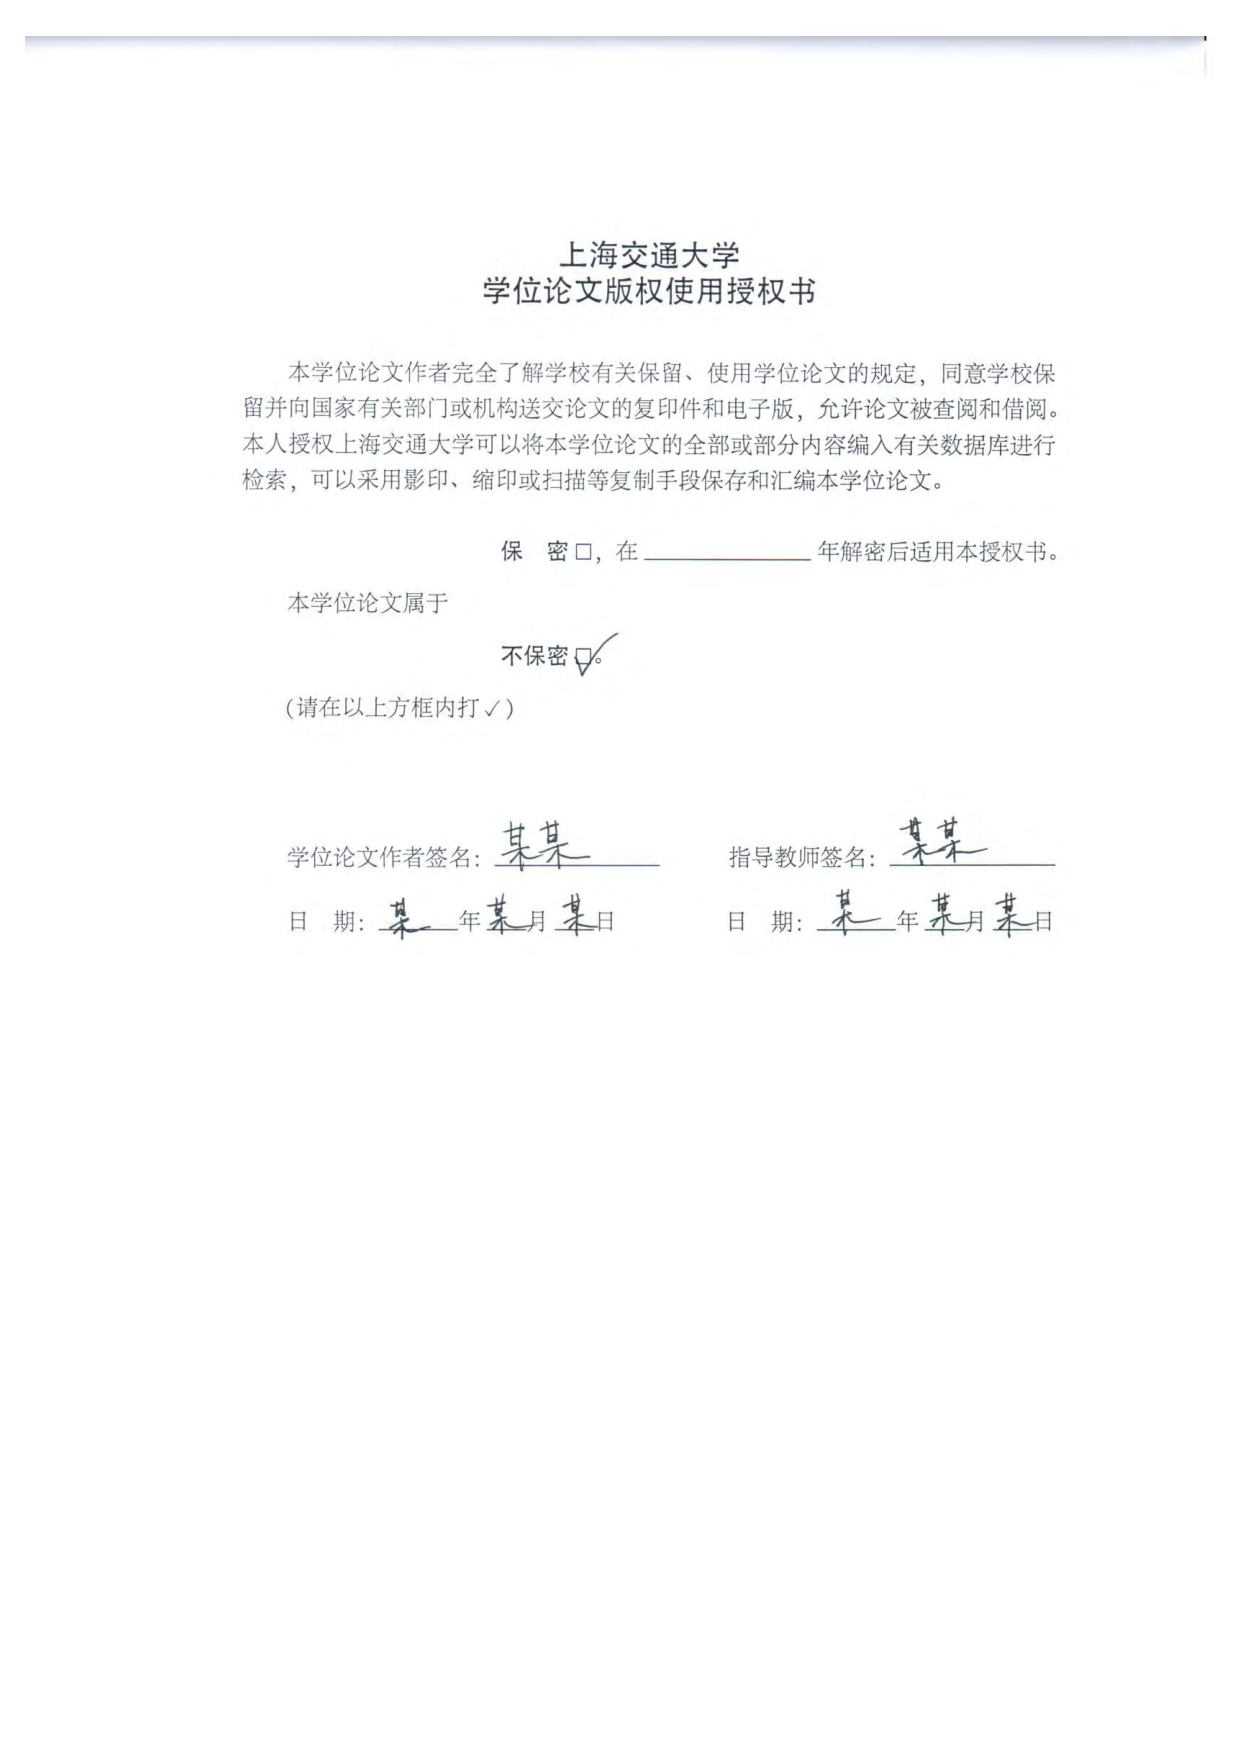
\includepdf{pdf/authorization.pdf}
	\cleardoublepage
\else
	\makeDeclareOriginal
	\makeDeclareAuthorization
\fi
\makeatother


\frontmatter 	% 使用罗马数字对前言编号

%% 摘要
\pagestyle{main}
%# -*- coding: utf-8-unix -*-
%%==================================================
%% abstract.tex for SJTU Master Thesis
%%==================================================

\begin{abstract}

CEPC和国际直线对撞机(International Linear Collider,ILC)[10]相仿,都主要利用希格斯韧致辐射(Higgstrahlung,ZH)过程产生希格斯粒子。相比于 LHC 上的质子-质子对撞,正负电子对撞机具有极低的本底,可以提供提供干净的希格斯事例,是精确研究希格斯粒子性质的理想场所。CEPC 的另一巨大优势是可以利用 Z 玻色子反冲质量法来研究希 格斯粒子,只需测量Z玻色子的衰变产物即可探测希格斯粒子。这种方法可以实现模型无关的精确测量,得到希格斯粒子的绝对衰变分支比和耦合常数,与 LHC 的实验结果合并后可以获得最优的结果。反冲质量法还可用于研究末态包含无法直接观测粒子的希格斯衰变道,从而寻找希格斯衰变中可能出现的暗物质和奇异新粒子等。


\keywords{\large 中国未来环形对撞机 \quad 希格斯粒子 \quad 衰变分支比}
\end{abstract}

\begin{englishabstract}

Precise measurement of the Higgs boson properties are important issues for the Circular Electron-Positron Collider(CEPC) project to understand the particles mass generation mechanism which strongly related to the coupling with the Higgs boson. CEPC experiments exclude the large area of the predicted Higgs mass region and their results indicate that Higgs boson mass will be light. 

Even if LHC discovers the Higgs like particle by the end of 2012, Higgs will be identified by the high precision measurement of the Higgs boson properties in CEPC and also Higgs measurement verifies the correctness of standard model (SM) or gives some hints toward its beyond. 

In this study, we evaluate the measurement accuracies of Higgs branching fraction to the H $\to$ $b\bar{b}$, $c\bar{c}$ and $gg$ at the center-of-mass energy of 250 GeV. Only the Monte Carlo samples are used in our analysis.


\englishkeywords{\large CEPC, Higgs Bosons, Higgs branching fraction}
\end{englishabstract}



%% 目录、插图目录、表格目录
\tableofcontents
\listoffigures
\addcontentsline{toc}{chapter}{\listfigurename} %将插图目录加入全文目录
\listoftables
\addcontentsline{toc}{chapter}{\listtablename}  %将表格目录加入全文目录
% \listofalgorithms
% \addcontentsline{toc}{chapter}{算法索引}        %将算法目录加入全文目录

%%# -*- coding: utf-8-unix -*-
\chapter{主要符号对照表}
\label{chap:symb}

\begin{longtable}{rl}
$\epsilon$     & 介电常数 \\
 $\mu$ 		& 磁导率 \\
 $\epsilon$     & 介电常数 \\
 $\mu$ 		& 磁导率 \\
 $\epsilon$     & 介电常数 \\
 $\mu$ 		& 磁导率 \\
 $\epsilon$ 	& 介电常数 \\
 $\mu$ 		& 磁导率 \\
 $\epsilon$     & 介电常数 \\
 $\mu$ 		& 磁导率 \\
 $\epsilon$     & 介电常数 \\
 $\mu$ 		& 磁导率 \\
 $\epsilon$     & 介电常数 \\
 $\mu$ 		& 磁导率 \\
 $\epsilon$ 	& 介电常数 \\
 $\mu$ 		& 磁导率 \\
 $\epsilon$     & 介电常数 \\
 $\mu$ 		& 磁导率 \\
 $\epsilon$     & 介电常数 \\
 $\mu$ 		& 磁导率 \\
 $\epsilon$     & 介电常数 \\
 $\mu$ 		& 磁导率 \\
 $\epsilon$ 	& 介电常数 \\
 $\mu$ 		& 磁导率 \\
 $\epsilon$     & 介电常数 \\
 $\mu$ 		& 磁导率 \\
 $\epsilon$     & 介电常数 \\
 $\mu$ 		& 磁导率 \\
 $\epsilon$     & 介电常数 \\
 $\mu$ 		& 磁导率 \\
 $\epsilon$ 	& 介电常数 \\
 $\mu$ 		& 磁导率 \\
 $\epsilon$     & 介电常数 \\
 $\mu$ 		& 磁导率 \\
 $\epsilon$     & 介电常数 \\
 $\mu$ 		& 磁导率 \\
 $\epsilon$     & 介电常数 \\
 $\mu$ 		& 磁导率 \\
 $\epsilon$ 	& 介电常数 \\
 $\mu$ 		& 磁导率 \\
 $\epsilon$     & 介电常数 \\
 $\mu$ 		& 磁导率 \\
 $\epsilon$     & 介电常数 \\
 $\mu$ 		& 磁导率 \\
 $\epsilon$     & 介电常数 \\
 $\mu$ 		& 磁导率 \\
 $\epsilon$ 	& 介电常数 \\
 $\mu$ 		& 磁导率 \\
 $\epsilon$     & 介电常数 \\
 $\mu$ 		& 磁导率 \\
 $\epsilon$     & 介电常数 \\
 $\mu$ 		& 磁导率 \\
 $\epsilon$     & 介电常数 \\
 $\mu$ 		& 磁导率 \\
\end{longtable}
 % 主要符号、缩略词对照表

\mainmatter	% 使用阿拉伯数字对正文编号

%% 正文内容
\pagestyle{main}
%# -*- coding: utf-8-unix -*-
%%==================================================
%% chapter01.tex for SJTU Bachelor Thesis
%%==================================================

%\bibliographystyle{sjtu2}%[此处用于每章都生产参考文献]
\chapter{Introduction}
\label{chap:1}

\section{Overview of the Phyiscs Case for CEPC}

This is a introduction

\section{Higgs Phyiscs at CEPC}

\section{Objective of Experiment}

\section{Chapter Summary}

%# -*- coding: utf-8-unix -*-
%%==================================================
%% chapter02.tex for SJTU Bachelor Thesis
%%==================================================

%\bibliographystyle{sjtu2}%[此处用于每章都生产参考文献]
\chapter{CEPC Experiment Detector}
\label{chap:2}

\section{Vertex Detector}

\section{Silicon Tracker}

\section{Main Tracking Detector - TPC}

\section{Calorimeter System}

\section{Muon System}

\section{Detector Magnet System}

\section{Chapter Summary}

%# -*- coding: utf-8-unix -*-
%%==================================================
%% chapter01.tex for SJTU Master Thesis
%%==================================================

%\bibliographystyle{sjtu2}%[此处用于每章都生产参考文献]
\chapter{Data Analysis}
\label{chap:3}

We will talk about the event selection in this chapter.

\section{Monte Carlo Sample}

The signal channel are $e^+e^-\to ZH \to\nu\nu(b\bar{b},c\bar{c},gg)$. In present work, almost all backgrounds are included in analysis.
They are the two/four fermions($\ell\ell$, $qq$, $\ell\ell\nu\nu$, $\ell\ell\ell\ell$, $qq\ell\ell$, $qq\nu\nu$, $qqqq$, $qq\ell\nu$) and other Higgs channel ($e^+e^-H$ and $\mu^+\mu^-H$). The $\tau^+\tau^- H$ samples haven't been included yet.
\begin{table}[!htb]
\centering
\begin{tabular}{c|c|c|c}
Name                           &Statistics             & weight& Note \\
$\nu\nu H$                     &5000fb$^{-1}$          &1      &  Full simulation\\
$(qq,e^+e^-,\mu^+\mu^-)H$      &5000fb$^{-1}$          &1      &  Full simulation\\
$\tau^-\tau^+H$                &0                      &0      &  Not available \\
2fermions/4fermions            &500fb$^{-1}$           &10     &  Fast simulation\\
\end{tabular}
\caption{MC sample}\label{MCSample}
\end{table}

\subsection{Signal}
Our signal comes from two parts.
\subsubsection{Leptonic}
Leptonic

\subsubsection{Hadronic}
Hadronic
\subsection{Two Fermions Background}

\subsection{Four Fermions Background}

\subsubsection{ZZ Process}
\subsubsection{WW Process}
\subsubsection{Single Z Process}
\subsubsection{Single W Process}
\subsubsection{Z or W Mixing Process}


\section{Event Selection}

\subsection{Preliminary Cut}
\subsubsection{$qq$}
\subsubsection{$qq\nu\nu$}
\subsubsection{$qq\ell\nu$}
\subsubsection{$qq\ell\ell$}
\subsubsection{$qqqq$}
\subsubsection{$\ell\ell$}
\subsubsection{$\ell\ell\ell\ell$}
\subsubsection{$\ell\ell\nu\nu$}
\subsubsection{$\ell{\ell}h$}
\subsubsection{$qqh$}
\subsubsection{$\nu{\nu}h$}
\subsubsection{Summary for Pre-Cut}

\subsection{Multi-Variable Analysis}

\subsection{Flavor Tagging}

\subsection{Template Fit}

\section{Chapter Summary}


%# -*- coding: utf-8-unix -*-
%%==================================================
%% chapter04.tex for SJTU Master Thesis
%%==================================================

%\bibliographystyle{sjtu2}%[此处用于每章都生产参考文献]
\chapter{Summary and Conclusion}
\label{chap:4}

This is the summary.


\appendix	% 使用英文字母对附录编号,重新定义附录中的公式、图图表编号样式
\renewcommand\theequation{\Alph{chapter}--\arabic{equation}}	
\renewcommand\thefigure{\Alph{chapter}--\arabic{figure}}
\renewcommand\thetable{\Alph{chapter}--\arabic{table}}
\renewcommand\thealgorithm{\Alph{chapter}--\arabic{algorithm}}

%% 附录内容,本科学位论文可以用翻译的文献替代。
%%# -*- coding: utf-8-unix -*-
\chapter{搭建模板编译环境}

\section{安装TeX发行版}

\subsection{Mac OS X}

Mac用户可以从MacTeX主页\footnote{\url{https://tug.org/mactex/}}下载MacTeX 2015。
也可以通过brew包管理器\footnote{\url{http://caskroom.io}}安装MacTeX 2015。

\begin{lstlisting}[basicstyle=\small\ttfamily, numbers=none]
brew cask install mactex
\end{lstlisting}

\subsection{Linux}

建议Linux用户使用TeXLive主页\footnote{\url{https://www.tug.org/texlive/}}的脚本来安装TeXLive 2015。
以下命令将把TeXLive发行版安装到当前用户的家目录下。
若计划安装一个供系统上所有用户使用的TeXLive,请使用root账户操作。

\begin{lstlisting}[basicstyle=\small\ttfamily, numbers=none]
wget http://mirror.ctan.org/systems/texlive/tlnet/install-tl-unx.tar.gz
tar xzvpf install-tl-unx.tar.gz
cd install-tl-20150411/
./install-tl
\end{lstlisting}

\section{安装中文字体}

\subsection{Mac OS X、Deepin}

Mac和Deepin用户双击字体文件即可安装字体。

\subsection{RedHat/CentOS用户}

RedHat/CentOS用户请先将字体文件复制到字体目录下,调用fc-cache刷新缓存后即可在TeXLive中使用新字体。

\begin{lstlisting}[basicstyle=\small\ttfamily, numbers=none]
mkdir ~/.fonts
cp *.ttf ~/.fonts				# 当前用户可用新字体
cp *.ttf /usr/share/fonts/local/	# 所有用户可以使用新字体
fc-cache -f
\end{lstlisting}



\backmatter	% 文后无编号部分 

%% 参考资料
%\printbibliography[heading=bibintoc]
\printbibliography

%% 致谢、发表论文、申请专利、参与项目、简历
%% 用于盲审的论文需隐去致谢、发表论文、申请专利、参与的项目
\makeatletter

%%
% "研究生学位论文送盲审印刷格式的统一要求"
% http://www.gs.sjtu.edu.cn/inform/3/2015/20151120_123928_738.htm

% 盲审删去删去致谢页
\ifsjtu@review\relax\else
  %# -*- coding: utf-8-unix -*-
\begin{thanks}

Thanks for my advisor Prof. Liang Li!

Thanks for Prof. Gang Li, Hao Liang in IHEP and Jianping Dai in INPAC!

Thanks for all the people in INPAC and IHEP!



\end{thanks}
 	  %% 致谢
\fi

% 盲审论文中,发表学术论文及参与科研情况等仅以第几作者注明即可,不要出现作者或他人姓名
\ifsjtu@review\relax
  %# -*- coding: utf-8-unix -*-

\begin{publications}{99}
    \item\textsc{第一作者}. {中文核心期刊论文}, 2007.  
    \item\textsc{第一作者}. {EI国际会议论文}, 2006.
\end{publications}

  %# -*- coding: utf-8-unix -*-

\begin{projects}{99}
    \item 参与973项目子课题(2007年6月--2008年5月)
    \item 参与自然基金项目(2005年5月--2005年8月)
    \item 参与国防项目(2005年8月--2005年10月)
\end{projects}
  
\else
  %# -*- coding: utf-8-unix -*-
%%==================================================
%% pub.tex for SJTUThesis
%% Encoding: UTF-8
%%==================================================

\begin{publications}{99}
    \item\textsc{Chen H, Chan C~T}. {Acoustic cloaking in three dimensions using acoustic metamaterials}[J]. Applied Physics Letters, 2007, 91:183518.
    \item\textsc{Chen H, Wu B~I, Zhang B}, et al. {Electromagnetic Wave Interactions with a Metamaterial Cloak}[J]. Physical Review Letters, 2007, 99(6):63903.
\end{publications}
	      %% 发表论文
  %# -*- coding: utf-8-unix -*-
%%==================================================
%% projects.tex for SJTUThesis
%% Encoding: UTF-8
%%==================================================

\begin{projects}{99}
    \item 973项目“XXX”
    \item 自然基金项目“XXX”
    \item 国防项目“XXX”
\end{projects}
  %% 参与的项目
\fi

% %# -*- coding: utf-8-unix -*-
\begin{patents}{99}
    \item 第一发明人,“永动机”,专利申请号202510149890.0
\end{patents}
	  %% 申请专利
% \include{tex/resume}	  %% 个人简历
\makeatother

\end{document}
